% !TEX root = ../main.tex

\section{Experimental setup}

This section provides geometric dimensions and typical operating conditions for the entrained flow reactor. Characteristics for the Blend3 and forest residue feedstocks are also discussed.

\subsection{Entrained flow reactor}

Fast pyrolysis in the TCPDU system occurs in the entrained flow reactor (EFR) which is comprised of a series of horizontal and vertical pipes connected with 90 degree elbows (see Figure \ref{fig:efr-assembly}). The EFR is essentially a pneumatic conveyor where biomass particles flow through a long pipe with several bends. Dimensions and material information about the EFR are provided in Figure \ref{fig:efr-geometry} below. Operating conditions such as temperatures, pressures, and flow rates for the EFR are shown in Figure \ref{fig:efr-flow}. Nitrogen gas at 500$^{\circ}$C is generally used as the conveying medium for the solids.

\begin{figure}[H]
	\centering
	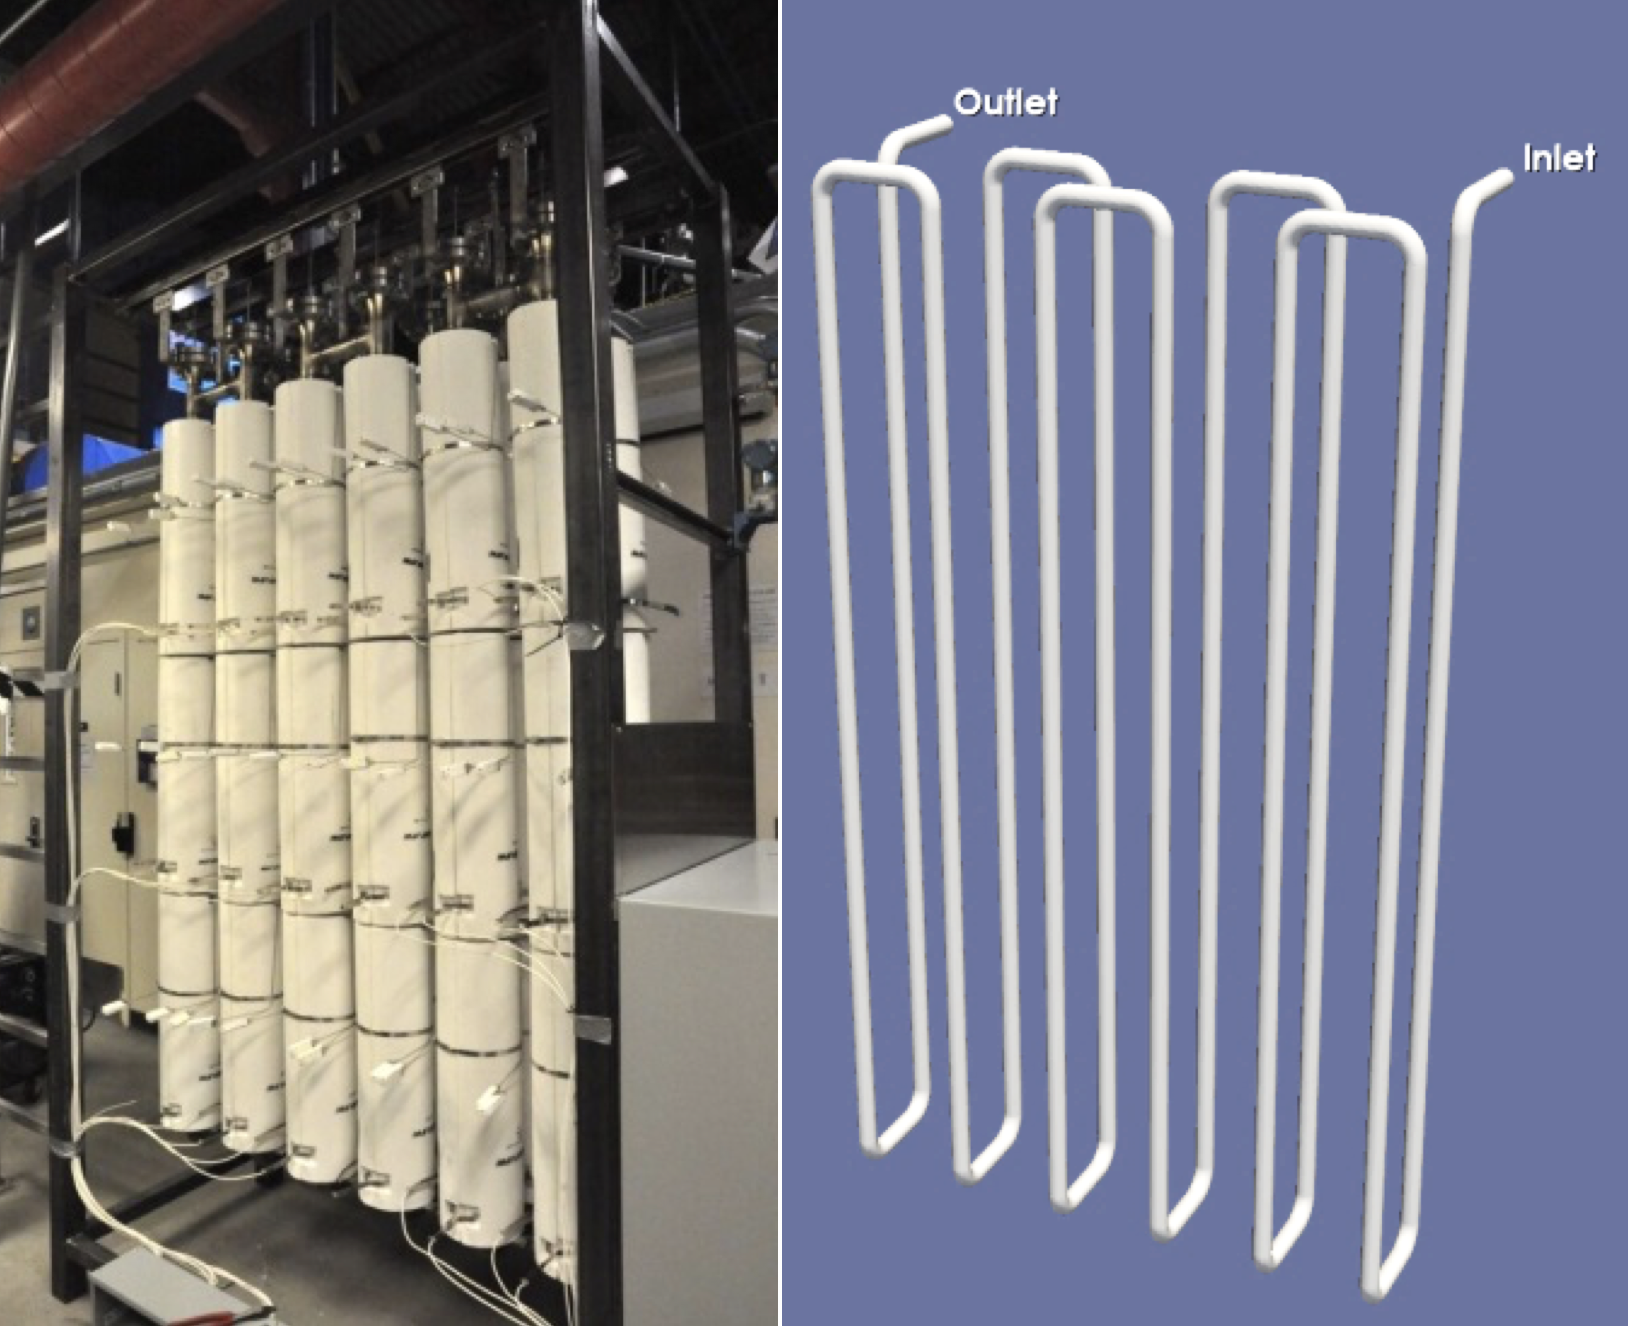
\includegraphics[width=0.8\textwidth]{figures/efr-assembly.png}
	\caption{Left - picture of the EFR assembly with heat jackets, insulation, and thermocouples. Right - CAD representation of the EFR pipe assembly used for MFiX simulations.}
	\label{fig:efr-assembly}
\end{figure}

\begin{figure}[H]
	\centering
	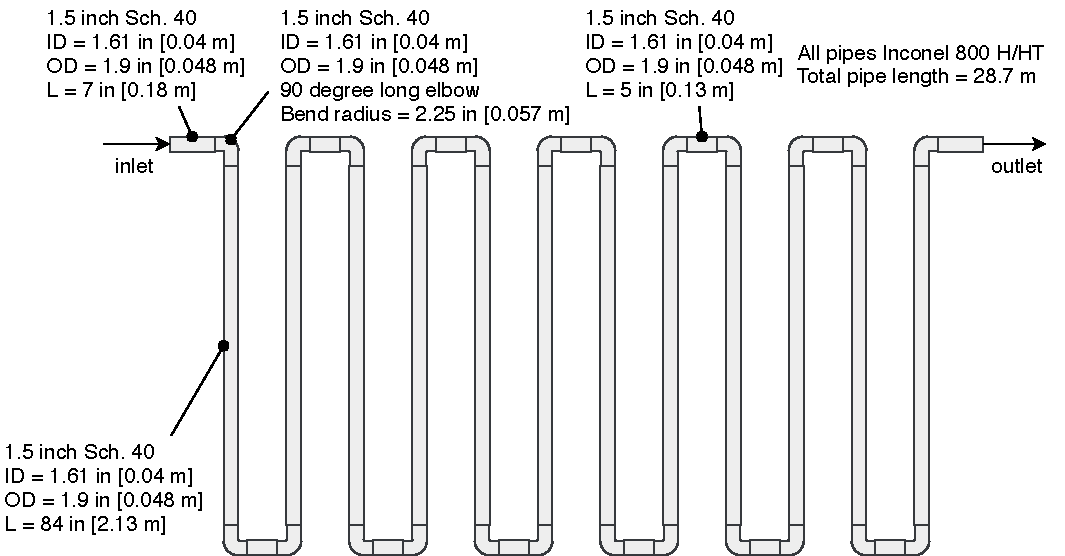
\includegraphics[width=\textwidth]{figures/efr-geometry.pdf}
	\caption{Geometry of the entrained flow reactor at NREL.}
	\label{fig:efr-geometry}
\end{figure}

\begin{figure}[H]
	\centering
	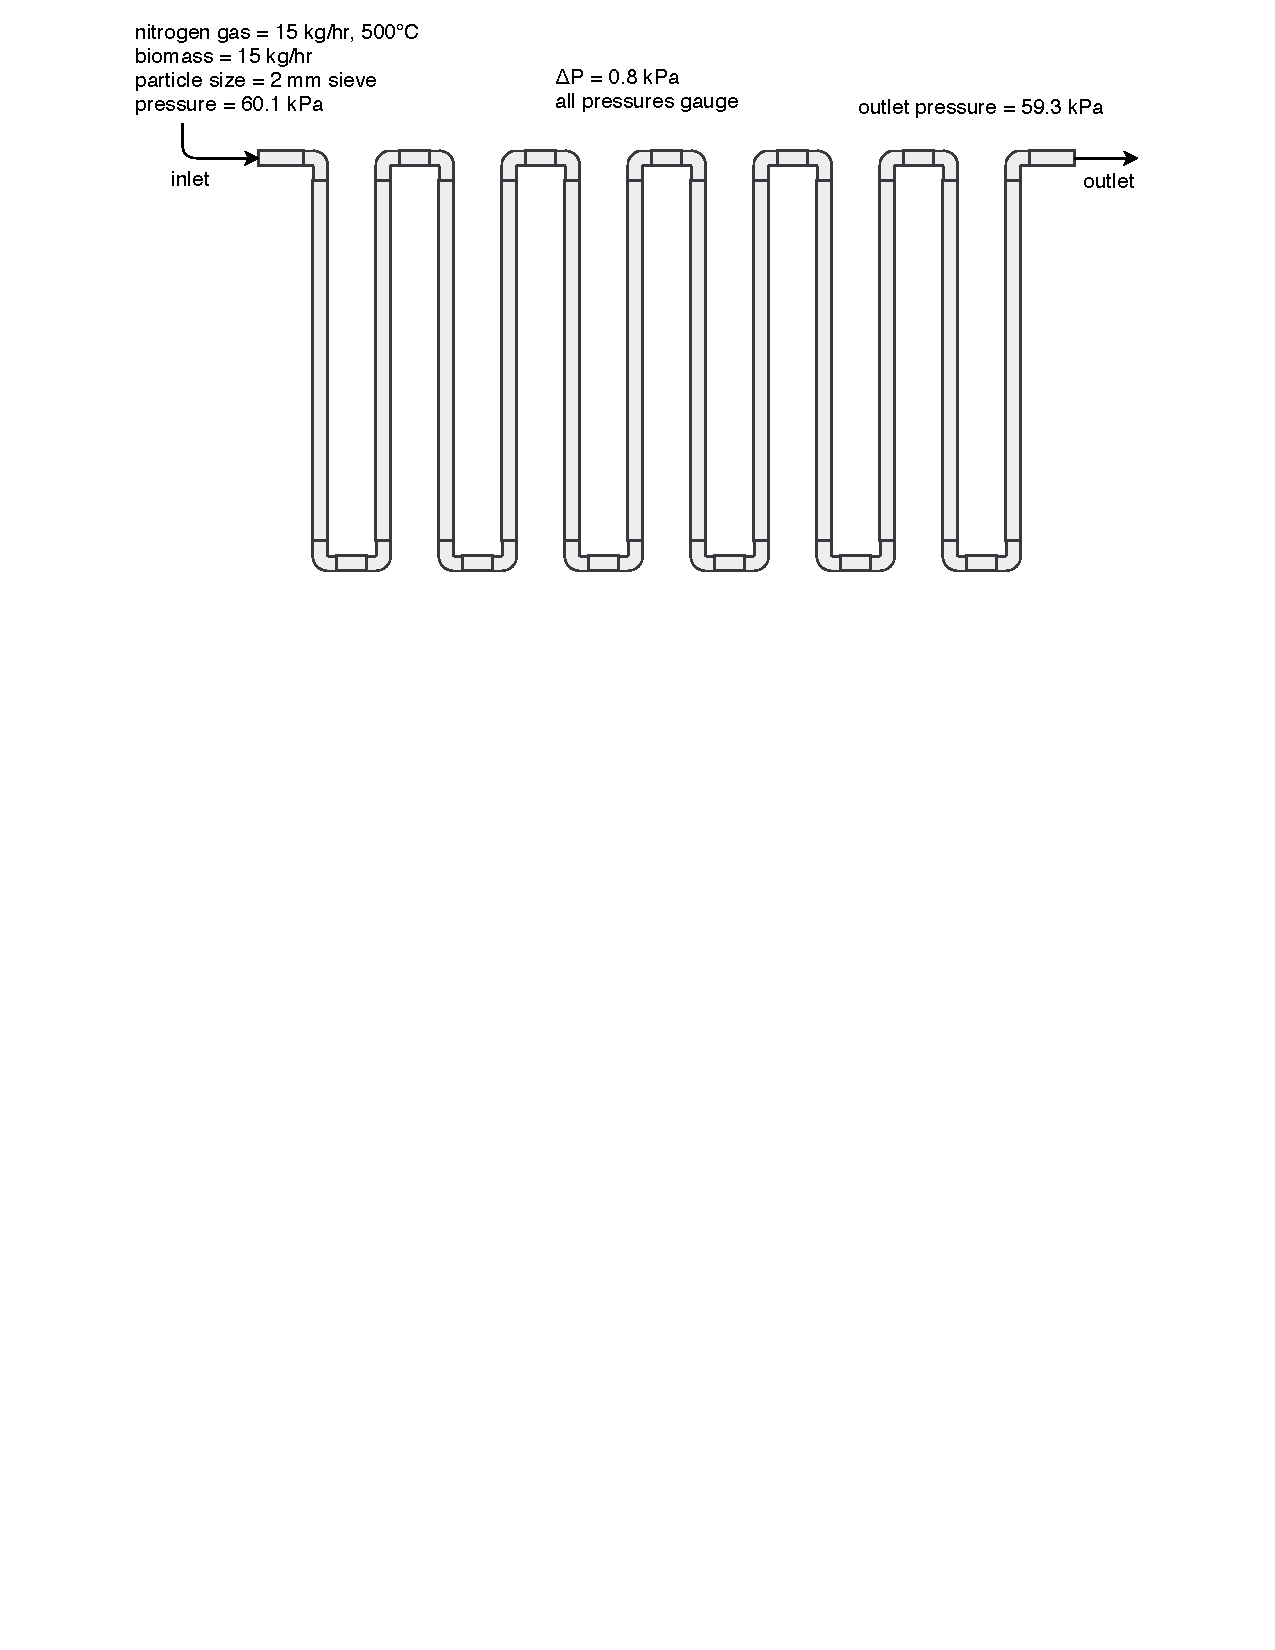
\includegraphics[width=\textwidth]{figures/efr-flow.pdf}
	\caption{Typical operating conditions for the entrained flow reactor.}
	\label{fig:efr-flow}
\end{figure}

\subsection{Blend3 feedstock}

General information about the Blend3 feedstock used in the entrained flow reactor is provided in Table \ref{tab:blend3-info}. There is currently no information regarding identification of the feedstock or who performed the feedstock measurements and data preparation. Proximate and ultimate analysis data for the feedstock are presented in Tables \ref{tab:blend3-prox} and \ref{tab:blend3-ult}. Only one set of analysis data is available therefore the uncertainty in the values is unknown.

\begin{table}[H]
    \centering
    \caption{General information for the Blend3 feedstock.}
    \label{tab:blend3-info}
    \begin{tabular}{ll}
        \toprule
        Item    & Description \\
        \midrule
        Name    & Blend3 \\
        ID      & ? \\
        Contact & ? \\
        \bottomrule
    \end{tabular}
\end{table}

\begin{table}[H]
    \centering
    \caption{Blend3 proximate analysis mass percent, as-received basis. Source \cite{Choratch-2017}.}
    \label{tab:blend3-prox}
    \begin{tabular}{lrrr}
        \toprule
        Proximate & \% ar & \% ar & \% ar \\
        \midrule
        FC        & 16.92 & ? & ? \\
        VM        & 76.40 & ? & ? \\
        ash       & 0.64  & ? & ? \\
        moisture  & 6.04  & ? & ? \\
        \bottomrule
    \end{tabular}
\end{table}

\begin{table}[H]
    \centering
    \caption{Blend3 ultimate analysis mass percent, as-received basis. Source \cite{Choratch-2017}.}
    \label{tab:blend3-ult}
    \begin{tabular}{lrrr}
        \toprule
        Element & \% ar & \% ar & \% ar \\
        \midrule
        C        & 49.52   & ? & ? \\
        H        & 5.28    & ? & ? \\
        O        & 38.35   & ? & ? \\
        N        & 0.15    & ? & ? \\
        S        & 0.02    & ? & ? \\
        ash      & 0.64    & ? & ? \\
        moisture & 6.04    & ? & ? \\
        \bottomrule
    \end{tabular}
\end{table}

The chemical analysis of the Blend3 feedstock is presented in Table \ref{tab:blend3-chem-analysis}. Again, only one set of data is available so the uncertainty in the measurements is unknown. The chemical analysis measurements are used to determine the biomass composition which is needed for the kinetics model.

\begin{table}[H]
    \centering
    \caption{Blend3 chemical analysis mass percent, dry basis. Source \cite{Starace-2020}.}
    \label{tab:blend3-chem-analysis}
    \begin{tabular}{lrrr}
        \toprule
        Chemical component & \% dry & \% dry & \% dry \\
        \midrule
        glucan                    & 38.95 & ? & ? \\
        acetyl                    & 1.59  & ? & ? \\
        arabinan                  & 1.40  & ? & ? \\
        galactan                  & 3.16  & ? & ? \\
        mannan                    & 10.52 & ? & ? \\
        xylan                     & 7.89  & ? & ? \\
        lignin                    & 29.48 & ? & ? \\
        free fructose             & 0.07  & ? & ? \\
        free glucose              & 0.04  & ? & ? \\
        sucrose                   & 0.04  & ? & ? \\
        water extractives         & 2.75  & ? & ? \\
        ethanol extractives       & 3.49  & ? & ? \\
        non-structural inorganics & 0.22  & ? & ? \\
        structural inorganics     & 0.41  & ? & ? \\
        \bottomrule
    \end{tabular}
\end{table}

\begin{table}[H]
    \centering
    \caption{Blend3 ash analysis as weight percent of ash. Source \cite{Choratch-2017}.}
    \begin{tabular}{lrrr}
        \toprule
        Metal oxide & wt. \% & wt. \% & wt. \% \\
        \midrule
        SiO$_2$     & 28.1 & ? & ? \\
        Al$_2$O$_3$ & 7.06 & ? & ? \\
        TiO$_2$     & 0.34 & ? & ? \\
        CaO         & 21.8 & ? & ? \\
        Na$_2$O     & 0.71 & ? & ? \\
        K$_2$O      & 13.8 & ? & ? \\
        P$_2$O$_5$  & 5.47 & ? & ? \\
        SO$_3$      & 1.23 & ? & ? \\
        Cl          & 0.09 & ? & ? \\
        CO$_2$      & 5.14 & ? & ? \\
        \bottomrule
    \end{tabular}
\end{table}

\begin{table}[H]
    \centering
    \caption{Blend3 particle properties from pelletized crushed feedstock. The crushed feedstock is used in the entrained flow reactor.}
    \begin{tabular}{crlc}
        \toprule
        Property & Value & Description & Source \\
        \midrule
        $\rho$  & 1,050 kg/m$^3$ & particle density, daf basis & \cite{Pecha-2018} \\
        $\eta$  & 0.27           & particle porosity & \\
        $k$     & 0.23 W/mK      & thermal conductivity & \\
        \bottomrule
    \end{tabular}
\end{table}

\begin{table}[H]
    \centering
    \caption{Entrained flow reactor yields for Blend3 feedstock.}
    \begin{tabular}{lr}
        \toprule
        Yield & wt. \% \\
        \midrule
        total liquid   & 64.9 \\
        char           & 13.9 $\pm$ 0.1 \\
        gas            & 17.2 $\pm$ 0.2 \\
        mass balance   & 96.9 $\pm$ 1.5 \\
        carbon balance & 93.0 $\pm$ 1.0 \\
        \bottomrule
    \end{tabular}
\end{table}

\subsection{Forest residue feedstock}

The forest residue feedstock is comprised of branches/twigs, cambium, needles, bark, and whitewood. This feedstock is used in the NREL fluidized bed reactor (FBR) for the purposes of the FCIC project. The FBR is operated at fast pyrolysis conditions for the thermochemical conversion of biomass. The reactor is sometimes referred to as the 2FBR.

\begin{table}[H]
    \centering
    \caption{General information for the forest residue feedstock.}
    \begin{tabular}{ll}
        \toprule
        Item    & Description \\
        \midrule
        Name    & forest residue \\
        ID      & ? \\
        Contact & ? \\
        \bottomrule
    \end{tabular}
\end{table}

\begin{table}[H]
    \centering
    \caption{Bark ultimate analysis mass percent, dry ash-free basis. Source \cite{Unknown-2019}.}
    \begin{tabular}{lrrr}
        \toprule
        Element & \% daf & \% daf & \% daf \\
        \midrule
        C        & 48.27 & ? & ? \\
        H        & 5.72  & ? & ? \\
        N        & 0.52  & ? & ? \\
        \bottomrule
    \end{tabular}
\end{table}

\begin{table}[H]
    \centering
    \caption{Branches/twigs ultimate analysis mass percent, dry ash-free basis. Source \cite{Unknown-2019}.}
    \begin{tabular}{lrrr}
        \toprule
        Element & \% daf & \% daf & \% daf \\
        \midrule
        C        & 49.69 & ? & ? \\
        H        & 6.36  & ? & ? \\
        N        & 0.25  & ? & ? \\
        \bottomrule
    \end{tabular}
\end{table}

\begin{table}[H]
    \centering
    \caption{Cambium ultimate analysis mass percent, dry ash-free basis. Source \cite{Unknown-2019}.}
    \begin{tabular}{lrrr}
        \toprule
        Element & \% daf & \% daf & \% daf \\
        \midrule
        C        & 48.52 & ? & ? \\
        H        & 6.39  & ? & ? \\
        N        & 0.11  & ? & ? \\
        \bottomrule
    \end{tabular}
\end{table}

\begin{table}[H]
    \centering
    \caption{Needles ultimate analysis mass percent, dry ash-free basis. Source \cite{Unknown-2019}.}
    \begin{tabular}{lrrr}
        \toprule
        Element & \% daf & \% daf & \% daf \\
        \midrule
        C        & 48.59 & ? & ? \\
        H        & 5.92  & ? & ? \\
        N        & 1.22  & ? & ? \\
        \bottomrule
    \end{tabular}
\end{table}

\begin{table}[H]
    \centering
    \caption{Whitewood ultimate analysis mass percent, dry ash-free basis. Source \cite{Unknown-2019}.}
    \begin{tabular}{lrrr}
        \toprule
        Element & \% daf & \% daf & \% daf \\
        \midrule
        C        & 48.27 & ? & ? \\
        H        & 6.15  & ? & ? \\
        N        & 0.10  & ? & ? \\
        \bottomrule
    \end{tabular}
\end{table}

\begin{table}[H]
    \centering
    \caption{Whitewood biomass composition mass percent, dry basis. Source \cite{Unknown-2020}.}
    \begin{tabular}{lr}
        \toprule
        Component & \% dry \\
        \midrule
        Cellulose       & 38.04 \\
        Hemicellulose   & 24.2  \\
        \bottomrule
    \end{tabular}
\end{table}
